%ब
\chapter{Design of Referential Integrity Constraints in NoSQL
databases}
\label{c:solutions}

% As mentioned previously,  cloud column-oriented key-value \acp{DBMS} lack
% referential integrity constraints to maintain foreign key relationships,  as
% seen in traditional \acp{RDBMS},  due to its non-relational data model. 
% Moreover,  these cloud \acp{DBMS} do not normalise data nor maintain
% relationships.
Traditionally, referential
integrity constraints are imposed on data items of a database to maintain
foreign key relationships. These relationships are
 maintained by correctly identifying and preserving the data dependencies 
 existing between the data items.
% Traditionally, foreign key relationships are
% maintained by correctly identifying and preserving the data dependencies existing between data items in a database.
% These dependencies are maintained and  validated by imposing referential
% integrity constraints on data items. 
Most popular traditional \acp{RDBMS}
preserve such dependency information in their \texttt{System} tables or data
dictionaries.  These tables store the necessary information  which is required
to maintain valid dependencies. The information stored in such tables include table
names,  primary and foreign keys among others.
This can be seen in popular \acp{RDBMS} like  MS SQL Server,  PostgreSQL,
Oracle, and so on.  

For example,  in MS SQL Server 2000, \texttt{sysforeignkeys}
is a \texttt{System} table which stores the information of all 
foreign keys of every table in a database, and \texttt{sysreferences}
stores the mappings of  foreign keys to the referenced primary key columns
(\todo{\citep{sys:msdn}}).
Information in these \texttt{System} tables consist of  the
names of tables and its constraints,  unique identifiers of 
referenced and referencing columns,  among others. 
In PostgreSQL, such information is saved as views which contain the dependency
information of data items in a database.
The view \texttt{table\_constraints} contains the information for all the
constraints in every table owned by the current user. (\todo{\cite{}}). 
Similarly, Oracle uses a \texttt{SYSTEM} meta-database to hold such constraint
information.
 In general, \texttt{System} tables or views with information
about the existing dependencies  are looked up by these \acp{RDBMS} whenever
referential integrity checks are triggered \citep{sys:msdn}.


The solutions presented in this thesis save the dependency information as
metadata. This metadata contains relevant  information about  foreign
key relationships in keyspaces and primary keys of column families. It is
accessed whenever an operation is performed on the data and referential
integrity needs to be validated.


This chapter describes  four  solutions  that implement referential
integrity constraints in a cloud \ac{NoSQL} \ac{DBMS}.
Section~\ref{s:Metadata} describes the metadata used by the solutions 
 to store the dependency information.
 % Section~\ref{s:API} describes the design and implementation of the experimental
% API developed to integrate all the four
% solutions. 
% Section~\ref{s:sol1} describes  the first solution, which implements
% referential integrity constraints by saving metadata along with the actual data.
% Section~\ref{s:sol2} describes the second  solution where metadata is
% saved as a top row. Section~\ref{s:sol3} describes the third   
% solution which saves metadata separate from the actual data.   
% Section~\ref{s:sol4}  describes the fourth solution which saves metadata in a separate cluster.
% Finally, Section~\ref{s:solutions-summary} presents a brief summary of this
% chapter. 

\section{Metadata}\label{s:Metadata}
Metadata in \acp{DBMS} provide information about the data stored within the
databases.
It may contain details related to schemas, constraints,  primary and foreign keys, and
so on.   As previously mentioned,  most traditional \acp{RDBMS} maintain such
metadata within their \texttt{System}  tables or data dictionaries.  
In Apache Cassandra, the \ac{DBMS} of interest, metadata is stored in a 
keyspace named \texttt{System} and it contains information
about the cluster and its nodes along with information related to the
keyspaces, column families, and so on (\todo{cite BOOK}).
 Even when Cassandra has a  \texttt{System} keyspace to store metadata, it 
 is read-only and hence it cannot be modified to store additional metadata
 about referential integrity constraints. 
%  As
% previously mentioned ,  most traditional \acp{RDBMS}
% maintain such metadata within their \texttt{System} tables or data dictionaries.
% Such metadata is decoupled from the actual data and its operations,  so that
% retrieving the metadata is faster since it does not involve handling the actual
% data(\todo{cite Duval}). 
% It has been studied that the \ac{DaaS} is moving towards maintaining metadata in
% the cloud \acp{DBMS},  where commonly this metadata stores information about the
% nodes in a distributed cluster (\todo{cite Bin(2010)}).  For  maintaining the
% scalability required in such cloud \acp{DBMS}, metadata is often decoupled from
% the actual data so that accessing metadata does not cause a bottleneck in
% performance.  Cassandra maintains  metadata about the nodes in a
% cluster  in a separate keyspace named \texttt{System}, which stores the
% properties of every node, for example the node tokens,  the name of the
% cluster to which  nodes belongs to, information about the stored keyspaces and
% column families and so on(\todo{cite BOOK}). 
% As per the design of Cassandra,  the \texttt{System} keyspace cannot be modified
% and thus  the metadata for the   solutions cannot be incorporated in this
% \texttt{System} keyspace.  Hence,  for preserving the metadata in each 
% solution implements a  different strategy In other words, metadata is associated
% with actual data in different ways.  Associations can be classified as
% (\todo{cite Duval}):
Hence,  for preserving the metadata, each 
solution implements a  different strategy in which metadata is associated
with actual data. Solutions~1 and~2 use embedded metadata, that is, metadata
is created with the actual data (\todo{cite Duval2009}); while solutions~3 and~4
associate metadata separately from the actual data.  Notice that, the structure
 of the metadata is kept the same across all the solutions even when  the way of
 storing and associating this metadata is different in each. 

The role of metadata in  the solutions is primarily to hold the necessary
 information required to maintain referential integrity. The metadata contains  
 information about primary keys,   foreign keys,  referenced and referencing
 column family details, constraints, and others.  The constraints considered in
 the solutions can be either \ac{PK} or \ac{FK} 
constraints. \ac{PK}
constraints specify which column is the primary key of a column family, while 
\ac{FK} constraints (or referential integrity constraints) determine the
foreign key relationship between two column families, that is, the
 column of a column family which  is dependent on the primary key  column of
 another column family.  Hence, for each column family with a primary key,  the
metadata  contains one \ac{PK} constraint  and  as
many \ac{FK} constraints as foreign key relationships. 
% Notice that, throughout
%  the solutions, the structure of metadata containing these constraints is
% consistent despite.  

The structure of the metadata is shown in
Figure~\ref{f:metadataInSolutions}.  This structure contains information about a
University keyspace example in which  a simple schema is applied for the
keyspace. In this example,  the details of the students are saved in  the
\texttt{Student} column family and the course
 details in the \texttt{Course} column family.
 The enrolment details of students are saved in the 
\texttt{Enrolment} column family by associating students to courses and
hence having foreign key relationships to both \texttt{Student} and
\texttt{Course} column families.
All the column families have unique primary keys and their \ac{PK} constraints are saved in
the metadata as presented in Figure~\ref{f:metadataInSolutions}, while the
foreign key relationships between \texttt{Enrolment}, \texttt{Student} and
\texttt{Course} are saved as \ac{FK} constraints.  For instance, consider in
 Figure~\ref{f:metadataInSolutions} the \ac{PK} constraint \texttt{CONST100},
 for the \texttt{Student} column family, and the \ac{FK} constraint  
 \texttt{CONST400} for the foreign key relationship between
\texttt{Enrolment} and \texttt{Student}.

\begin{figure}[h]
	\centering
	
	\newcolumntype{C}{@{\hspace{2.5pt}}>{\scriptsize}c@{\hspace{2.5pt}}}
	\begin{tabular}{CCC CCC CC}
		\toprule
		\bfseries ConstraintName & \bfseries Keyspace & \bfseries ConstraintType &
		\bfseries ColumnFamily & \bfseries RKeyspace & \bfseries RConstraintName &
		\bfseries RColumn & \bfseries DeleteRule\\
		\midrule
		CONST100 & University & P & Student & University & & StudentId &\\
		\rc CONST200 & University & P & Course & University & & CourseId &\\
		CONST300 & University & P & Enrolment & University & & RowId &\\
% 		\hline
% 		\hline
		\rc CONST400 & University & R & Enrolment & University & CONST100 & StudentId
		& CASCADE\\
		CONST500 & University & R & Enrolment & University & CONST200 & CourseId &
		NODELETE\\
		\rc CONST600 & University & F & Course & University & CONST500 & CourseId &
		NODELETE\\
		CONST700 & University & F & Student & University & CONST400 & StudentId &
		CASCADE\\
		\bottomrule
	\end{tabular}
	\caption{Metadata for the Solutions}\label{f:metadataInSolutions}
\end{figure}


Specifically, the structure of the metadata contains:

\begin{itemize}
  
  \item \texttt{ConstraintName:} is the name assigned for
  every constraint and it uniquely identifies an
  existing \ac{PK} or \ac{FK} constraint in the metadata. 
   For example,  \texttt{CONST100} and \texttt{CONST400} are the
  \texttt{ConstraintNames}.
  
  \item \texttt{Keyspace:}represents the name of the Keyspace the constraint
  belongs to. 
  
  \item \texttt{ConstraintType:} denotes the type of the constraint and the
  possible values are '\texttt{P}', '\texttt{R}' and '\texttt{F}'.
%   The former referes to  a \ac{PK} constraint while the latter represents  a
%    \ac{FK} constraint. 
	A \ac{PK} constraint is referred by '\texttt{P}' while '\texttt{R}' and
	'\texttt{F}' are two representations of \ac{FK} constraints.
		'\texttt{R}' represents the Referential Integrity
	Constraint (or the \ac{FK} constraint) a child entity has on a parent primary
	key and '\texttt{F}' shows the  existing dependencies on a parent
	entity.
	For example, \texttt{CONST400} shows that the the parent entity
	 for \texttt{Enrolment} is \texttt{Student}. \texttt{CONST700}
	shows that parent entity \texttt{Student} has child dependencies on it. Notice
	that, the constraint type '\texttt{F}'
	is primarily used to locate the child dependencies for a parent when it
	is deleted or updated.
% 	\begin{itemize}
% 	  \item  '\texttt{P}' represents a \ac{PK} constraint
% 	  \item '\texttt{R}' represents a 

   
  \item \texttt{ColumnFamily:} refers to the column family this constraint
  exists in. For example,  the \ac{PK} constraint
  \texttt{CONST100}  exists in column family \texttt{Student} and the column
  family of the \ac{FK} constraint \texttt{CONST400}
  is \texttt{Enrolment}.
  
  \item \texttt{RKeyspace:}is the name of the keyspace on which this constraint
  is applied.  In the example, constraints  are applied in  the keyspace
  \texttt{University}.
  
    %   In other words, it indicates which primary key
%   is referenced or which . 
  \item \texttt{RConstraintName:} For \ac{FK}
  constraints, \texttt{RConstraintName} represents the constraint that is
  referenced. For constraint type '\texttt{R}' this represents the referenced
  \ac{PK} constraint and for constraint type '\texttt{F}' it shows  the child
  dependencies for a parent entity. In the example, the \ac{FK} constraint
  \texttt{CONST400} references the \ac{PK} constraint \texttt{CONST100},  which
  means that \texttt{Enrolment} has a foreign key relationship with
  \texttt{Student}.
   In \texttt{CONST700} this field indicates that \ac{FK} constraint
   \texttt{CONST400} exists for \texttt{Student}. Notice that in a \ac{PK}
   constraint this field is left blank since it has no references to other keys.
  
  \item \texttt{RColumn:}  indicates the primary key column on which this
  constraint is applicable.  For \ac{PK} constraints,  this holds the name of
  the primary key column. For \ac{FK} constraints, this field denotes
  the referenced column.  This example shows that the \ac{PK} constraint
  \texttt{CONST100} is applied on the primary key column \texttt{StudentId} of
  \texttt{Student} column family . The \ac{FK} constraint \texttt{CONST400}
  shows that the referenced column is \texttt{StudentId},  indicating that
  \texttt{Enrolment} references  primary key column \texttt{StudentId} of
  \texttt{Student}.
  
  \item \texttt{DeleteRule:}stores the type of data manipulation rule applicable
  on this constraint. The possible values are  \texttt{Cascade} and
  \texttt{NoDelete}.  This field is not applicable  for \ac{PK} constraints
   since data manipulation rules are associated with constraints that hold
  dependency information like the \ac{FK} constraints.
  
\end{itemize}

Metadata in the solutions are accessed whenever referential integrity
validations are triggered to extract information about \ac{FK} constraints. 
% Specific methods are designed in all the solutions to retrieve and process the
% metadata in order to validate referential integrity. 
Each solution stores metadata in a distinct way and provides specific methods to
access and process the metadata to support the validation. The way these
solutions store metadata and the motivation behind the design of its metadata
storage is presented in the following sections.

\section{Solution1:  Metadata with Special Characters} \label{s:design-sol1}

% \subsection{Metadata Storage}
	This solution saves the metadata embedded with the actual data and is stored in
	the column family belonging to the actual data. This means that metadata is
	included in every super column in a column family and is stored as the 
	value of column \texttt{Metadata}. Since metadata is common for all the entities in an entity
	class, every super column contains the same metadata value for this column.For
	example, in the University keyspace, metadata in \texttt{Student} is stored in
	every super column as seen in Figure~\ref{fd:Metadata-Solution1}.
	
% 		\begin{figure}[H]
% 			\centering
% 			%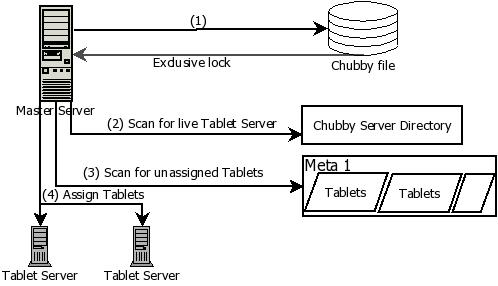
\includegraphics[width=5cm,   height=5cm]{. /figure/random. jpg}
% 			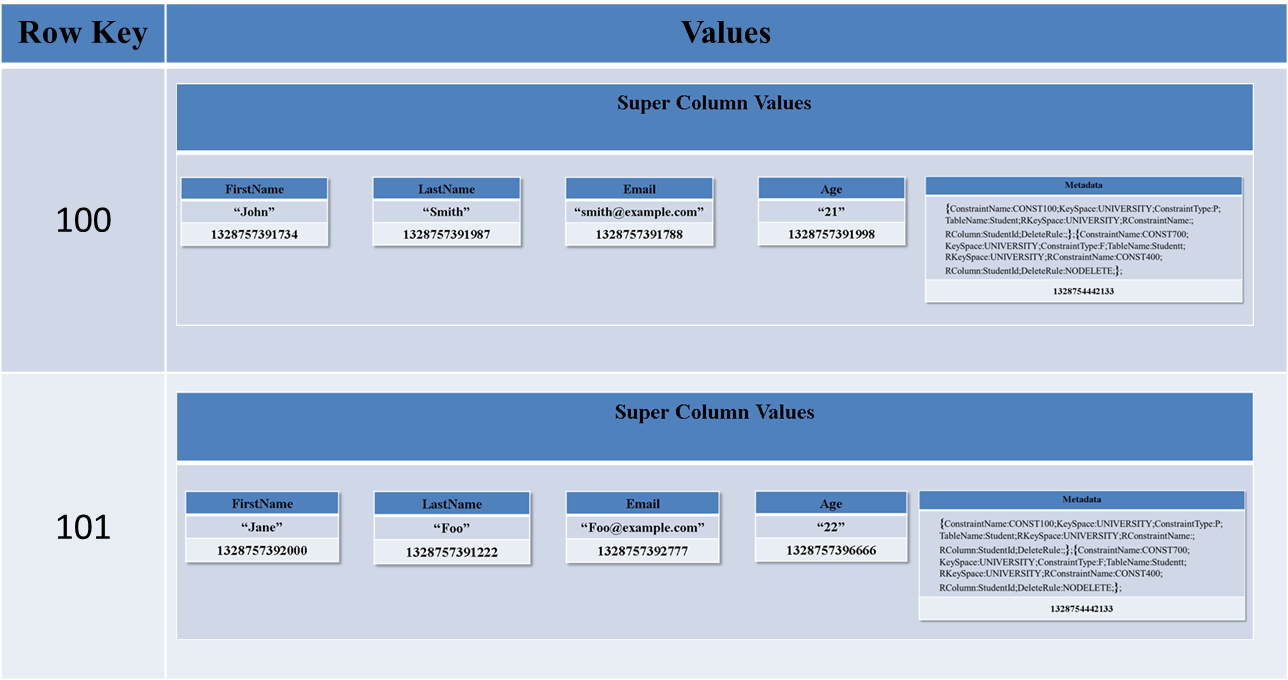
\includegraphics[width=1\textwidth]{./figure/Solutions/Sol1-MD-ColumnFamily.png}
% 			\caption{Metadata storage in Solution 1}\label{f:sol1-Student-md}
% 		\end{figure}
		
	In this solution, the structure of the constraints in metadata is as described
	in Section~\ref{s:Metadata} and each entity class stores  its \ac{PK}
	constraint and related \ac{FK} constraints in the metadata. 
	Each entity stores the following constraints as its metadata.
	
		\begin{itemize}
		  \item  \ac{PK} constraint showing the primary key of the column family.
		  \item \ac{FK} constraints 
				\begin{itemize}
					\item In the case of a parent entity the \ac{FK} constraints are the \ac{FK}
					constraints of type '\texttt{F}' to identify the child entities when the entity
					is being updated or deleted.
					\item  In the case of a child entity the \ac{FK} constraint of type '\texttt{R}'
					is stored to indicate the parent entities.
					\item If an entity is both a parent and a child, then its metadata
					stores its \ac{PK} constraint and the \ac{FK} constraints of both types.
				\end{itemize}
		\end{itemize}
		

	For instance, \texttt{Student}  is a parent entity with a child dependendent on
	it, namely \texttt{Enrolment}. 
	Its metadata thus contains its \ac{PK} constraint \texttt{CONST100} and the
	\ac{FK} constraint \texttt{CONST700}. Since
	\texttt{Enrolment} is a child entity it  stores its \ac{PK} constraint
	\texttt{CONST300} and its \ac{FK} constraints \texttt{CONST400} and
	\texttt{CONST500}. Similarly, other entities like \texttt{Course} store its
	\ac{PK} and respective \ac{FK} constraints.
	
		\begin{figure}[H] \label{fd:Metadata-Solution1}
			\centering
			\subfigure[Metadata Column]{
				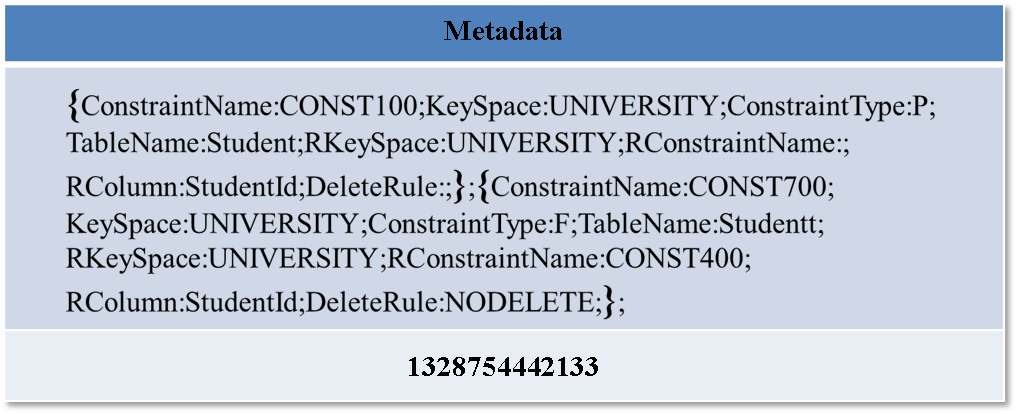
\includegraphics[width=.6\textwidth]{./figure/Solutions/Sol1-MD-Col.png}
	% 			\caption{Response Time for \texttt{insert}}\label{fr:response-insert}
			}
			\subfigure[Metadata in Supercolumns]{
				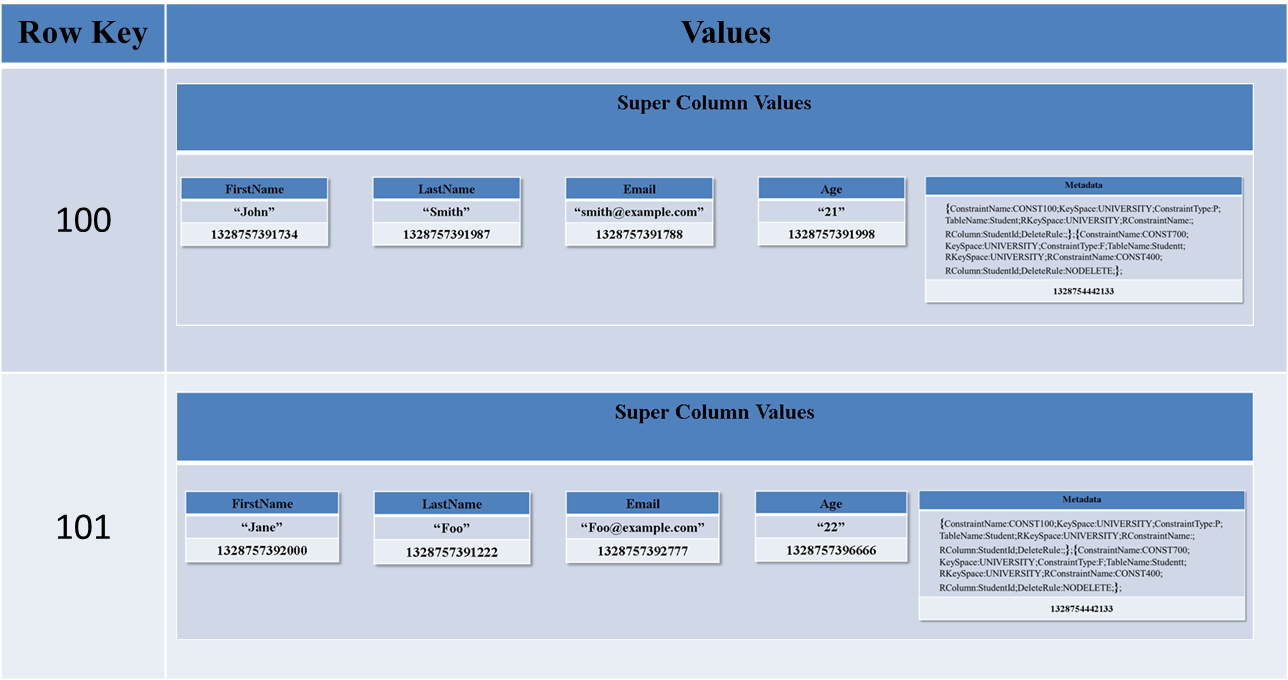
\includegraphics[width=1\textwidth]{./figure/Solutions/Sol1-MD-ColumnFamily.png}
	% 			\caption{Throughput}\label{fr:through-insert}
			} 
			\caption{Metadata storage in Solution 1}
		\end{figure}
	Special characters are used within the metadata to separate the constraints and
	to identify its different parts. The special characters used in this solution
	are '\texttt{\{}', '\texttt{\}}','\texttt{;}' and '\texttt{:}'. The special
	characters are used the following way:
	
	\begin{itemize}
	\item Each constraint is enclosed in curly brackets and separated from each
	other by the special character '\texttt{;}'. For example,in \texttt{Student}
	\texttt{CONST100} and \texttt{CONST700} are enclosed in curly braces and
	separated by '\texttt{;}'. Thus, '\texttt{\};}' marks the end of every
	constraint in the metadata.


	\item The different parts of each constraint are separated by the special character
	'\texttt{;}'. For example,  '\texttt{;}' separates the \texttt{ConstraintName}
	 and \texttt{Keyspace} and other parts in the constraints \texttt{CONST100} and
	 \texttt{CONST700}
	 
	 
	\item Each part and its value are separated by the special character
	'\texttt{:}'. For example, \texttt{ConstraintName} is separated from
	its value \texttt{CONST100} with a \texttt{:}. This helps in identifying the
	name and value for every part while parsing the metadata information
	in the \ac{API}.
	
	\end{itemize}






\section{Solution2:  Metadata as a Top Row} \label{s:design-sol2}
\section{Solution3:  Metadata Column Family} \label{s:design-sol3}
\section{Solution4:  Metadata Cluster} \label{s:design-sol4}



% These methods and all the
% solutions are incorporated  into an experimental \ac{API}, which is
% described in Chapter~\ref{c:Implementation}.
